% -*- TeX-master: "master.tex" -*-
\section{Introduction}

Two important questions in physics:
\begin{itemize}
\item What is matter made of?
  \begin{itemize}
  \item What are the elementary constituents?
  \end{itemize}
\item How do the elementary constituents interact?
  \begin{itemize}
  \item What are the forces and dynamics in Nature?
  \end{itemize}
\end{itemize}

Most popular media focus on the first question. In Fermilab's ``search for the top quark'', or the LHC ``quest for the Higgs boson'', focus is placed on the excitement of discovering new forms of matter.

This is fun, but what is really exciting is not garnering a new trophy, but in what the existance of these new particles implies for the second question --- what new dynamics must exist that this new particle can help reveal?

\subsection{The matter}
\begin{itemize}
\item Hydrogen:
  \begin{figure}[H]
    \centering
    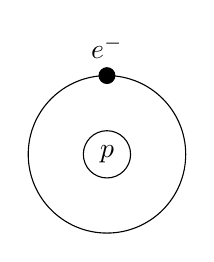
\begin{tikzpicture}{scale=1.5}
      \draw (0,0) circle [radius=0.3] node {$p$};
      \draw (0,0) circle [radius=1.0];
      \filldraw (0,1.0) circle [radius=0.1]
      node [yshift=1em] {$e^-$};
    \end{tikzpicture}
    \caption{Hydrogen Atom}
    \label{fig:hydrogen}
  \end{figure}
  A visualization is in fig~\ref{fig:hydrogen} Some properties of hydrogen:
  \begin{gather*}
    \text{Radius: } r_e\approx \SI{1}{\angstrom}\\
    \text{Binding Energy: }\SI{13}{\eV}
  \end{gather*}
  The unit of the binding energy is an Electron-Volt, which is what we will use for all energies for the duration of these notes.
  \begin{definition}[Electron-Volt]
    The electron volt is defined as the kinetic energy of an electron accelerated across a 1V potential, the usual SI unit prefixes can be applied such that 1keV=$10^3$eV, 1MeV=$10^6$eV etc.
  \end{definition}
\item Electron
  \begin{gather*}
    \text{Mass: } m_e= 0.511\text{ MeV}\\
    \text{Charge}=-1\\
    \text{Spin}=\frac12
  \end{gather*}
\item Proton
  \begin{gather*}
    \text{Mass: } m_p= 938\text{ MeV}\approx 1\text{ GeV}\\
    \text{Charge}=+1\\
    \text{Spin}=\frac12
  \end{gather*}
  \item Neutron
  \begin{gather*}
    \text{Mass: } m_n= m_p+1.3\text{ MeV}\approx m_p\\
    \text{Charge}=0\\
    \text{Spin}=\frac12
  \end{gather*}
  \item Deuterium is a Hydrogen with a neutron
\end{itemize}

\paragraph{Sizes}
\begin{itemize}
\item The electron is effectively a point
\item The nucleons, which are protons and neutrons have a ``radius'' of $\sim 10^{-15}$m, which is given the name of $1$fm, a ``Fermi'' or femtometer, which is notably less than the scale of hydrogen
\end{itemize}

\subsection{Forces in play:}
\begin{itemize}
\item Gravity $\sim$ negligible:
  \begin{align*}
    F=G_N\frac{m_p m_e}{r^2}
  \end{align*}
\item Electric:
  \begin{align*}
    F=\frac{e^2}{4\pi}\frac{Q_p Q_e}{r^2}
  \end{align*}
\item Strong --- Binds nucleons into nuclei
\item Weak --- Causes nuclear ``beta'' decay, and fusion
\end{itemize}

\subsection{Beta ($\beta$) decay}
A Process described by:
\begin{align*}
  n\to p+e^{-}+\bar{\nu}_e
\end{align*}
Where $\bar{\nu}_e$ is an anti-electron neutrino. This process has a lifetime $\tau$ of $14$ minutes.

Note that $m_n-m_p>m_e$

\paragraph{Q/ Why doesn't deuterium decay?} In short, conservation of energy, since $2m_p+m_e+m_{\nu_e}=1877.05$MeV, however, the mass of deuterium is $m_d=1876.64$. The masses are not large enough to allow for this decay:
\begin{figure}[H]
  \centering
  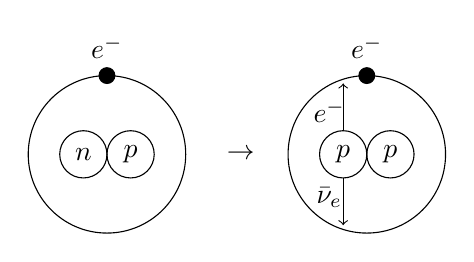
\begin{tikzpicture}
    \draw (0,0) circle [radius=0.3] node {$n$};
    \draw (0.6,0) circle [radius=0.3] node {$p$};
    \draw (0.3,0) circle [radius=1.0];
    \filldraw (0.3,1.0) circle [radius=0.1]
    node [yshift=1em] {$e^-$};
    \node at (2.0,0) {$\cancel{\rightarrow}$};
    \draw (3.3,0) circle [radius=0.3] node {$p$};
    \draw (3.9,0) circle [radius=0.3] node {$p$};
    \draw (3.6,0) circle [radius=1.0];
    \filldraw (3.6,1.0) circle [radius=0.1]
    node [yshift=1em] {$e^-$};
    \draw[->] (3.3,-0.3) to (3.3,-0.9) node [yshift=1em] {\hspace{-1em}$\bar{\nu}_e$};
    \draw[->] (3.3,0.3) to (3.3,0.9) node [yshift=-1em] {\hspace{-1em}$e^{-}$};
  \end{tikzpicture}
  \caption{Theoretical Deuterium Decay}
\end{figure}

\paragraph{Neutrinos and $\beta$ decay}
The other interesting story of $\beta$ decay is regarding the neutrino. In 1930, Chadwick observed the decay of tritium: $^3$H $\to\ ^3$He$+e^-$. Strangely, the $e^-$ was \emph{not} monoenergetic, as conservation of energy and momentum would require. This was catastrophic, and confronted with experimental evidence, many were prepared to throw out energy conservation. Pauli proposed a ``desperate remedy'' that some invisible particle must be carrying the energy away. Fermi's theory of weak interactions described this particle as a ``neutrino'' (little neutral one), and successfully described $\beta$ decay.

\textbf{Note}: The neutrino in $\beta$ decay was later found to be an antiparticle.

\begin{itemize}
\item Neutrinos then can be added to our list of ``matter''
  \begin{align*}
    \SI{0.01}{\eV}\leq m_{\nu_e}\leq\SI{1.4}{\eV}
  \end{align*}
  A consequence of this mass is that we can take neutrinos to be kinematically massless.
\end{itemize}

\subsection{Antiparticles}
Every particle has an antiparticle with opposite quantum numbers, but identical mass and spin:
\begin{itemize}
\item The electron $e^-$ has the positron $e^+$
\item The proton $p$ has the antiproton $\bar{p}$
\item The neutron $n$ has the antineutron $\bar{n}$
\item And the neutrinos $\nu$ have the antineutrinos $\bar{\nu}$ as we have seen
\end{itemize}
These (specifying the electron neutrino and its antiparticle) compose $\sim100\%$ of all the \textbf{observed} matter in the universe, though are only $5\%$ of the total matter.

Up to this point we have used chemistry and nuclear physics, particle physics picks up at the next level of depth.

\subsection{Quarks}
As it turns out, the proton and neutron are \textbf{not} fundamental.

If you perform a Rutherford-like scattering experiment at large energies (short distance), you find that protons and neutrons are composed of 3 hard spheres, called ``constituent quarks''

In fact, we go a bit deeper and find:
\begin{itemize}
\item The up quark $u$ and the up antiquark $\bar{u}$
\item The down quark $d$ and the down antiquark $\bar{d}$
\end{itemize}

These were ``predicted'' by Gell-Mann and Zweig as an explanation for apparent relationships between other particles, but we are getting ahead of ourselves.

The new particles we can add to our list of matter is:

\begin{itemize}
\item Up quark
  \begin{gather*}
    \text{Mass: } m_u= 4\text{ MeV} \ll m_p\\
    \text{Charge}=+\frac23\\
    \text{Spin}=\frac12
  \end{gather*}
\item Down quark
  \begin{gather*}
    \text{Mass: } m_d= 7\text{ MeV} \ll m_p\\
    \text{Charge}=-\frac13\\
    \text{Spin}=\frac12
  \end{gather*}
\end{itemize}
Note the odd fractional charge that both of these quarks have.

We can then think of $p,\bar{p}$ and $n,\bar{n}$ as:
\begin{figure}[H]
  \centering
  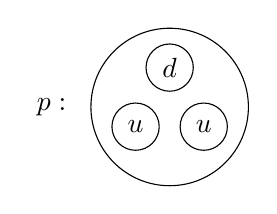
\begin{tikzpicture}
    \node at (0,0) {$p:$};
    \draw (1.500, 0.00) circle (1.0);
    \draw (1.500, 0.50) circle (0.3) node {$d$};
    \draw (1.067,-0.25) circle (0.3) node {$u$};
    \draw (1.933,-0.25) circle (0.3) node {$u$};
  \end{tikzpicture}
  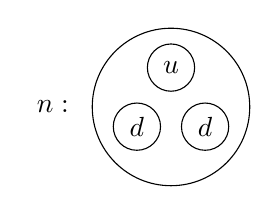
\begin{tikzpicture}
    \node at (0,0) {$n:$};
    \draw (1.500, 0.00) circle (1.0);
    \draw (1.500, 0.50) circle (0.3) node {$u$};
    \draw (1.067,-0.25) circle (0.3) node {$d$};
    \draw (1.933,-0.25) circle (0.3) node {$d$};
  \end{tikzpicture}
  \\
  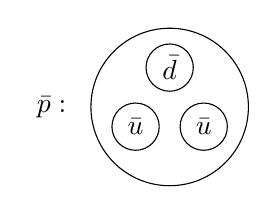
\begin{tikzpicture}
    \node at (0,0) {$\bar{p}:$};
    \draw (1.500, 0.00) circle (1.0);
    \draw (1.500, 0.50) circle (0.3) node {$\bar{d}$};
    \draw (1.067,-0.25) circle (0.3) node {$\bar{u}$};
    \draw (1.933,-0.25) circle (0.3) node {$\bar{u}$};
  \end{tikzpicture}
  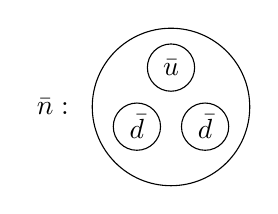
\begin{tikzpicture}
    \node at (0,0) {$\bar{n}:$};
    \draw (1.500, 0.00) circle (1.0);
    \draw (1.500, 0.50) circle (0.3) node {$\bar{u}$};
    \draw (1.067,-0.25) circle (0.3) node {$\bar{d}$};
    \draw (1.933,-0.25) circle (0.3) node {$\bar{d}$};
  \end{tikzpicture}
  \caption{Protons and Neutrons as Quarks}
\end{figure}

\subsection{Beta Decay Again}
We should revisit $\beta$ decay in terms of the constituent quarks of protons and neutrons. We instead see the process as:
\begin{figure}[H]
  \centering
  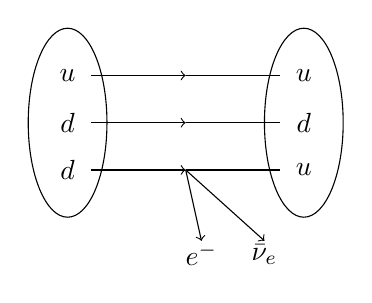
\begin{tikzpicture}
    \draw (0,0) ellipse (0.5 and 1.2);
    \node at (0, 0.6) {$u$};
    \node at (0, 0.0) {$d$};
    \node at (0,-0.6) {$d$};
    \draw (3,0) ellipse (0.5 and 1.2);
    \node at (3, 0.6) {$u$};
    \node at (3, 0.0) {$d$};
    \node at (3,-0.6) {$u$};
    \draw[->] (0.3, 0.6) to (1.5, 0.6);
    \draw[-]  (1.5, 0.6) to (2.7, 0.6);
    \draw[->] (0.3, 0.0) to (1.5, 0.0);
    \draw[-]  (1.5, 0.0) to (2.7, 0.0);
    \draw[->] (0.3,-0.6) to (1.5,-0.6);
    \draw[-]  (1.5,-0.6) to (2.7,-0.6);
    \draw[->] (1.5,-0.6) to (1.7,-1.5) node [yshift=-0.5em] {$e^-$};
    \draw[->] (1.5,-0.6) to (2.5,-1.5) node [yshift=-0.5em] {$\bar{\nu}_e$};
  \end{tikzpicture}
  \caption{$\beta$ decay in terms of quarks}
  \label{fig:beta}
\end{figure}
Thus we can describe the Fermi weak interaction in terms of quarks:
\begin{figure}[H]
  \centering
  \begin{tikzpicture}
    \begin{feynhand}
      \vertex (a) at (0,0) {$d$};
      \vertex (i) at (1.5,0);
      \vertex (b) at (3,0) {$u$};
      \vertex (e) at (3,1.5) {$e^-$};
      \vertex (n) at (3,-1.5) {$\bar{\nu}_e$};
      \propag[fer] (a) to (i);
      \propag[fer] (i) to (b);
      \propag[fer] (i) to (e);
      \propag[antfer] (i) to (n);
    \end{feynhand}
  \end{tikzpicture}
  \caption{``Four-Fermion'' Fermi Interaction}
  \label{fig:fermi}
\end{figure}

Thus so far, our ``Standard Model'' looks just like:
\begin{gather*}
  \pmqty{u\\d}\\
  \pmqty{\nu_e\\e}
\end{gather*}

However, there is still more to come!

\subsection{Muon}
Denoted by $\mu^\pm$. In 1937 Neddermeyer and Anderson, and Street and Stevenson, found muons in showers of cosmic rays (particles hit the upper atmosphere, and produce heavy charged particles that reach the ground). Originally, they were thought to be particles predicted by Yukawa to mediate the strong force because their mass, $\SI{105}{\mega\eV}$ is close to that of the now known pion, $m_\pi\approx\SI{139}{\mega\eV}$. They were (poorly) called ``mu meons''.

The dominant decay of a muon suggests a 3-bpdyy decay:
\begin{align*}
  \mu^+\to e^+\nu_e\bar{\nu}_{?}
\end{align*}
The lack of observation of $\mu^+\to e^+\gamma$, and later in 1962 at the AGS, where Lederman, Schwartz, and Steinberger showed $\bar{\nu}_\mu+p\to\mu^++n$, but $\bar{\nu}+p\cancel{\to}e^++n$, in the inverse reaction, implied the existance of a muon neutrino.

\subsection{The Zoo}
By 1961, there were 27 ``fundamental'' strongly interacting particles known. Gell-Mann and Ne'eman independently noticed that adding a ``strange'' new quantum number, they could collect the particles into groups related by a simple symmetry --- $SU(3)$, which we'll discuss later.

By 1964, only one particle was missing --- one with 3 units of ``strangeness'':
\begin{figure}[H]
  \centering
  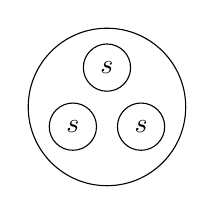
\begin{tikzpicture}
    \draw (1.500, 0.00) circle (1.0);
    \draw (1.500, 0.50) circle (0.3) node {$s$};
    \draw (1.067,-0.25) circle (0.3) node {$s$};
    \draw (1.933,-0.25) circle (0.3) node {$s$};
  \end{tikzpicture}
  \caption{Theoretical ``Strange'' Particle}
  \label{fig:strange}
\end{figure}
This particle is predicted to have spin $\frac32$ and charge $-1$. They also preduced the mass $\SI{1.7}{\giga\eV}$, and lifetime. In 1964, the $\Omega^-$ was discovered at Brookhaven National Lab.

\begin{itemize}
\item The effects of this new periodic table called ``The Eightfold Way'' were profound. The concept of symmetry as \emph{the} central theoretical device was established --- and we are still paying that price\ldots
\item Later Gell-Mann and Zweig proposed the quark model of 3 flavors: up, down, strange. By 1970 this model was in trouble.
\item Free quarks had not been observed.
\item The weak decay $s\cancel{\to}d\nu\bar{\nu}$ did not appear. Glashow, Iliopoulos, and Maiani proposed a ``charming'' solution to the latter. Adding a fourth quark with charge $+\frac23$ would allow for a symmetry to forbid these ``neutral current'' decays. 
\item In 1974 BNL and SLAC each discovered a $c\bar{c}$-bound state, called the $J/\psi$. The lifetime of $\SI{e-20}{\s}$ was 1000 times longer than for strange particles.
\item It seemed clear that the number of quarks $=$ the number of leptons
\end{itemize}
This gives a new standard model:
\begin{gather*}
  \pmqty{u\\d}\quad\qquad\pmqty{c\\s}\\
  \underbrace{\pmqty{\nu_e\\e}}_{1^{\text{st}}\text{ Generation}}
  \underbrace{\pmqty{\nu_\mu\\\mu}}_{2^{\text{nd}}\text{ Generation}}
\end{gather*}
The new additions are:
\begin{itemize}
\item Charm quark: $m_c\approx\SI{1.25}{\GeV}\gg m_u$
\item Strange quark: $m_d\approx\SI{95}{\MeV}\gg m_d$
\item Muon: $m_\mu=\SI{105.658369}{\MeV}\gg m_e$
\item Muon neutrino: $m_{\nu_\mu}\approx m_{\nu_e}\approx0$
\end{itemize}

The second generation particles are \emph{unstable}:
\begin{figure}[H]
  \centering
  \begin{tikzpicture}
    \begin{feynhand}
      \vertex (a) at (0,0) {$c$};
      \vertex (i) at (1.5,0);
      \vertex (b) at (3,0) {$s$};
      \vertex (e) at (3,1.5) {$e^+$};
      \vertex (n) at (3,-1.5) {$\nu_e$};
      \propag[fer] (a) to (i);
      \propag[fer] (i) to (b);
      \propag[fer] (i) to (e);
      \propag[antfer] (i) to (n);
    \end{feynhand}
  \end{tikzpicture}
  \begin{tikzpicture}
    \begin{feynhand}
      \vertex (a) at (0,0) {$c$};
      \vertex (i) at (1.5,0);
      \vertex (b) at (3,0) {$s$};
      \vertex (e) at (3,1.5) {$\mu^+$};
      \vertex (n) at (3,-1.5) {$\nu_\mu$};
      \propag[fer] (a) to (i);
      \propag[fer] (i) to (b);
      \propag[fer] (i) to (e);
      \propag[antfer] (i) to (n);
    \end{feynhand}
  \end{tikzpicture}
  \\
  \begin{tikzpicture}
    \begin{feynhand}
      \vertex (a) at (0,0) {$s$};
      \vertex (i) at (1.5,0);
      \vertex (b) at (3,0) {$u$};
      \vertex (e) at (3,1.5) {$e^-$};
      \vertex (n) at (3,-1.5) {$\bar{\nu}_e$};
      \propag[fer] (a) to (i);
      \propag[fer] (i) to (b);
      \propag[fer] (i) to (e);
      \propag[antfer] (i) to (n);
    \end{feynhand}
  \end{tikzpicture}
  \begin{tikzpicture}
    \begin{feynhand}
      \vertex (a) at (0,0) {$s$};
      \vertex (i) at (1.5,0);
      \vertex (b) at (3,0) {$u$};
      \vertex (e) at (3,1.5) {$\mu^-$};
      \vertex (n) at (3,-1.5) {$\bar{\nu}_\mu$};
      \propag[fer] (a) to (i);
      \propag[fer] (i) to (b);
      \propag[fer] (i) to (e);
      \propag[antfer] (i) to (n);
    \end{feynhand}
  \end{tikzpicture}
  \\
  \begin{tikzpicture}
    \begin{feynhand}
      \vertex (a) at (0,0) {$\mu^-$};
      \vertex (i) at (1.5,0);
      \vertex (b) at (3,0) {$\nu_\mu$};
      \vertex (e) at (3,1.5) {$e^-$};
      \vertex (n) at (3,-1.5) {$\bar{\nu}_e$};
      \propag[fer] (a) to (i);
      \propag[fer] (i) to (b);
      \propag[fer] (i) to (e);
      \propag[antfer] (i) to (n);
    \end{feynhand}
  \end{tikzpicture}
  \caption{Second Generation Decays}
  \label{fig:gentwo}
\end{figure}
In 1975 the $\tau$ lepton was discovered at SLAC in $e^+e^-\to\tau^+\tau^-$. Immediate searches began for third generation particles:
\begin{itemize}
\item 2001 DONUT at Fermilab observed $\nu_\tau$ events in emulsion
\item 1977 a $b\bar{b}$-bound state called the upsilon was discovered at Fermilab, $m_b\approx\SI{5}{\GeV}$
\item There \emph{had} to be a sixth quark of mass $m_t<\SI{45}{\GeV}$, no $\SI{80}{\GeV}$, no $\SI{110}{\GeV}$, no $\SI{140}{\GeV}$. WHERE IS IT???
\item 1995 top quark discovered at Fermilab via its decay. Lifetime so short it forms \emph{no} bound states! $m_t\approx\SI{175}{\GeV}$. 
\end{itemize}
Thus we have the third generation:
\begin{gather*}
  \pmqty{u\\d}\hspace{0.5em}\pmqty{c\\s}\hspace{0.5em}\pmqty{t\\b}\\
  \pmqty{\nu_e\\e}\pmqty{\nu_\mu\\\mu}\pmqty{\nu_\tau\\\tau}
\end{gather*}
New additions:
\begin{itemize}
\item Top quark: $m_t=\SI{172.4}{\GeV}$
\item Bottom quark: $m_b=\SI{4.5}{\GeV}$
\item Tau: $m_\tau=\SI{1.78}{\GeV}$
\item Tau neutrino: $m_{\nu_\tau}\approx m_{\nu_e}\approx m_{\nu_\mu}\leq \SI{1}{\eV}$
\end{itemize}

\paragraph{Fourth Generation?}

There is no evidence for a fourth generation current, but if there were, we would expect:
\begin{gather*}
  m_{\nu_4}>40-\SI{45}{\GeV}\\
  m_{\ell_4}\geq\SI{100}{\GeV}\\
  m_{b'}\geq\SI{130}{\GeV}
\end{gather*}

\paragraph{Great Mysteries:}

\begin{itemize}
\item Why are there 3 generations?
\item Why do some mix and others not?
\item Why do masses range from $10^{-12}$ to $10^2$ \si{\GeV}?
\end{itemize}

\subsection{Forces (Interactions):}
Relativity and quantum mechanics lead to Quantum Field Theory.

There are 4 forces at play (kinda):
\begin{enumerate}
  \setcounter{enumi}{-1}
\item \emph{Gravity}, as mentioned, is simply too weak at the level of particles to observe. Therefore we'll ignore it (for now).
\item \emph{Electromagnetism}: Mediated by exchange of virtual bosons called photons, $\gamma$:
  \begin{gather*}
    \text{Mass: } m_\gamma= 0\\
    \text{Charge}=0\\
    \text{Spin}=1
  \end{gather*}
  Einstein's Nobel Prize was not for gravity, but for this 1905 argument that the electromagnetic field was quantized. Hence, light really could be though of as a particle with energy $E=h\nu$, and not just as a wave.

  In 1923, Compton showed that light scattered from a particle of mass $m$ had a wavelength shifted by $\lambda-\lambda'=\lambda_c(1-\cos\theta)$, with $\lambda_c=\frac{h}{mc}$-precisely what you get if $m_\gamma=0$ and is a particle.

  Photons (light) couple to anything that carries charge. So far that is $e^\pm$, $u$, $d$, $\bar{u}$, $\bar{d}$, and other generations.
\item \emph{Strong Force}: Mediated by gluons, $g$:
    \begin{gather*}
    \text{Mass: } m_g= 0\\
    \text{Charge}=0\\
    \text{Spin}=1
  \end{gather*}
  Quarks feel gluon force, leptons do not.

  Quarks carry \emph{color}=red, green, blue.

  Gluons have to bind strongly to overcome EM repulsion. They save the quark model by saying there are actually 3 quarks for each type: $u,d,s$ etc. Otherwise the $\Omega^-(sss)$  could not exist due to the Pauli exclusion principle. When $\Omega^-$ was found in 1964, Greenberg proposed the color model. There were strong lingering doubts about this solution until 1979 where PETRA at DESY produced 3 jets: $q,\bar{q},g$.

  \emph{Note}: There are 9 color combinations, but only 8 gluons, we'll return.
\item \emph{Weak Force}: Mediated by massive $W/Z$ Bosons.

  What we earlier called the ``Fermi interaction'' is really exchange of a heavy particle. Force is not intrinsically weak, just suppressed by $W$ mass:
  \begin{gather*}
    \text{Mass: } m_W= \SI{80.4}{\GeV}\\
    \text{Charge}=\pm1\\
    \text{Spin}=1
  \end{gather*}
  $W$ boson changed particle type or \emph{flavor}
\end{enumerate}

The underlying field theories behind each of these has a name:
\begin{itemize}
\item Electromagnetism: Quantum Electro Dynamics (QED)
\item Strong Force: Quantum Chromo Dynamics (QCD)
\item Weak Force: Quantum Flavor Dynamics (QFD)\footnote{This nomenclature however is rarely used.}
\end{itemize}
The Standard Model is described by \emph{Gauge Theory}, QED, QCD and QFD are all examples of gauge theories, based on ``local'' symmetries.

A gauge theory is described by a gauge ``group''
\begin{itemize}
\item QED
  \begin{align*}
    u\to \underbrace{e^{i\theta}}_{U(1)}u
  \end{align*}
  
\item QFD
  \begin{align*}
    \pmqty{u\\d}\to \underbrace{\pmqty{&&& \\ &&&}}_{2\times2:SU(2)}\pmqty{u\\d}
  \end{align*}
\item QCD
  \begin{align*}
    \pmqty{u_r\\u_g\\u_b}\to
    \underbrace{\pmqty{&&&&& \\ &&&&& \\ &&&&&}}_{3\times3:SU(3)}
    \pmqty{u_r\\u_g\\u_b}
  \end{align*}
\end{itemize}
Particles (fields) experience forces described by their transformation under these groups.

The Standard model group is: $SU(3)\times SU(2)\times U(1)$

Note that Gravity is \emph{not} a gauge theory.

There are two types of symmetry we would like to include in our theory of the universe, global and local ones.
\begin{definition}[Global Symmetry]
  A global symmetry is a symmetry that changes every point in the transformation space the same. For a rotation, the entire system would be shifted by some angle $\theta$.
\end{definition}
Global symmetries, while nice, give rise to a sort of action at a distance, which is something we want to avoid in our interpretation of the universe via Field Theory. This leads to a sense that the symmetries of the Standard Model are ``Local'' rather than global, hence the other type of symmetry to discuss
\begin{definition}[Local Symmetry]
  A non global symmetry is called a local symmetry, and is characterized by the transformation parameter having dependence on spacetime:
  \begin{gather*}
    \text{Global Parameter: }\theta\\
    \text{Local  Parameter: }\theta(x)
  \end{gather*}
\end{definition}

A Gauge theory is a theory of massless spin-one particles that transmit force.
\begin{itemize}
\item QED: $m_\gamma=0$
\item QCD: $m_g=0$
\item QFD: $M_W=\SI{80.4}{\GeV}$, whoops!
\end{itemize}
The Gauge Symmetry is apparently \emph{broken} (or Hidden).

\begin{remark}
  An analogous system is a ferromagnet:
  \begin{figure}[H]
    \centering
    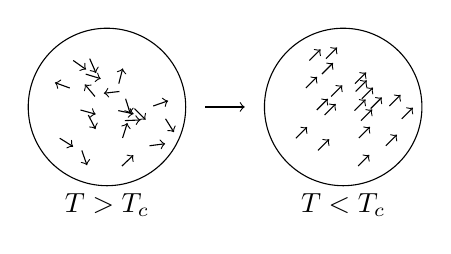
\begin{tikzpicture}
      \node at (0,-1.25) {$T>T_c$};
      \draw (0,0) circle (1.0);
      \draw[->] (0.34954, -0.0199438) to (0.490203, -0.162119);
      \draw[->] (0.150047, 0.296553) to (0.20043, 0.490102);
      \draw[->] (0.743747, -0.150205) to (0.850037, -0.319624);
      \draw[->] (0.198332, -0.393883) to (0.258539, -0.203161);
      \draw[->] (-0.335555, -0.038404) to (-0.14284, -0.0918898);
      \draw[->] (-0.152624, 0.13327) to (-0.281111, 0.286538);
      \draw[->] (0.236579, 0.104484) to (0.29672, -0.0862591);
      \draw[->] (-0.319563, -0.55186) to (-0.253705, -0.740706);
      \draw[->] (0.226788, -0.173314) to (0.426614, -0.164954);
      \draw[->] (-0.472952, 0.240987) to (-0.660934, 0.309271);
      \draw[->] (-0.428682, 0.59036) to (-0.265005, 0.475426);
      \draw[->] (0.143533, -0.0461538) to (0.339274, -0.0872084);
      \draw[->] (0.540831, -0.492648) to (0.739169, -0.466921);
      \draw[->] (-0.270044, 0.417371) to (-0.0786918, 0.359195);
      \draw[->] (-0.236663, -0.102218) to (-0.145731, -0.28035);
      \draw[->] (-0.599859, -0.396888) to (-0.430448, -0.50319);
      \draw[->] (0.190446, -0.749809) to (0.335538, -0.612156);
      \draw[->] (0.587397, 0.0124832) to (0.776281, 0.078231);
      \draw[->] (-0.219336, 0.613831) to (-0.138749, 0.430786);
      \draw[->] (0.158473, 0.196568) to (-0.0402765, 0.174242);
      \draw (3,0) circle (1.0);
      \node at (3,-1.25) {$T<T_c$};
      \draw[->] (3.34954, -0.0199438) to (3.49096, 0.121478);
      \draw[->] (3.15005, 0.296553) to (3.29147, 0.437974);
      \draw[->] (3.74375, -0.150205) to (3.88517, -0.00878408);
      \draw[->] (3.19833, -0.393883) to (3.33975, -0.252462);
      \draw[->] (2.66444, -0.038404) to (2.80587, 0.103017);
      \draw[->] (2.84738, 0.13327) to (2.9888, 0.274691);
      \draw[->] (3.23658, 0.104484) to (3.378, 0.245906);
      \draw[->] (2.68044, -0.55186) to (2.82186, -0.410439);
      \draw[->] (3.22679, -0.173314) to (3.36821, -0.0318922);
      \draw[->] (2.52705, 0.240987) to (2.66847, 0.382408);
      \draw[->] (2.57132, 0.59036) to (2.71274, 0.731782);
      \draw[->] (3.14353, -0.0461538) to (3.28495, 0.0952676);
      \draw[->] (3.54083, -0.492648) to (3.68225, -0.351226);
      \draw[->] (2.72996, 0.417371) to (2.87138, 0.558792);
      \draw[->] (2.76334, -0.102218) to (2.90476, 0.0392038);
      \draw[->] (2.40014, -0.396888) to (2.54156, -0.255467);
      \draw[->] (3.19045, -0.749809) to (3.33187, -0.608388);
      \draw[->] (3.5874, 0.0124832) to (3.72882, 0.153905);
      \draw[->] (2.78066, 0.613831) to (2.92209, 0.755253);
      \draw[->] (3.15847, 0.196568) to (3.29989, 0.33799);
      \draw[->] (1.25,0) to (1.75,0);
    \end{tikzpicture}
    \caption{Ferromagnet Symmetry Breaking}
    \label{fig:magnet}
  \end{figure}
  For $T>T_c$, there is clearly no preferred direction for the system, so for all intents and purposes it is rotationally symmetric. However as soon as we go below $T_c$, this symmetry is ``spontaneously'' broken.
\end{remark}

We do not know what ``breaks'' the symmetry $\implies$ \underline{new force of nature}.

The central question in particle physics today is to answer what new force exists, and what are the particles associated with it?

A second frontier: What is the origin of quark and lepton masses?

\subsection{Units in Particle Physics}
\begin{table}[H]
  \centering
  \begin{tabular}{c|c}
    Typical Energies & Sizes\\ \hline
    \si{\eV} $\sim10^{1} \si{\eV}$ & $\si{\nm}\sim10^{-9}\si{\m}$  \\
    \si{\keV}$\sim10^{3} \si{\eV}$ & $\si{\angstrom}\sim10^{-10}\si{\m}$  \\
    \si{\MeV}$\sim10^{6} \si{\eV}$ & $\si{\pm}\sim10^{-12}\si{\m}$  \\
    \si{\GeV}$\sim10^{9} \si{\eV}$ & $\si{\femto\m}\sim10^{-15}\si{\m}$  \\
    \si{\TeV}$\sim10^{12}\si{\eV}$
  \end{tabular}
  \caption{Typical Values in Particle Physics}
\end{table}

\begin{definition}[Natural Units]
  As a convention, factors of $\hbar$ and $c$ are set to be $1$, meaning they are dimensionless as well as valueless, so everything is measired in units of energy.

  The only conversion factors we need to know:
  \begin{align*}
    c&=\SI{3e8}{\m\per\s}\\
    \hbar c&=\SI{197}{\MeV\femto\m}
  \end{align*}
  These are the only values we need to memorize.
\end{definition}

Electric charge can get complicated with most authors either using Lorentz-Heaviside units:
\begin{align*}
  F=\frac{e^2}{4\pi}\frac{Q_e Q_p}{r^2}
\end{align*}
Or Gaussian (CGS) units:
\begin{align*}
  F=e^2\frac{Q_e Q_p}{r^2}
\end{align*}
The relationship between these is that $e_{LH}=\sqrt{4\pi}e_{CGS}$.

Again, memorize one thing, since we defined $\hbar c=1$, we have:
\begin{align*}
  \alpha&=\frac{e^2}{4\pi\hbar c}=\frac{e^2}{4\pi}\\
  &\approx\frac1{137}
\end{align*}
So that the force is simply:
\begin{align*}
  F=\frac{\alpha Q_e Q_p}{r^2}
\end{align*}
